\chapter{Multivaraite Classifiers developed for the effective lifetime measurement}
\label{sec:appendix2}
%Details of the input variables used and the development of the classifiers.
%What need to go into here ...
%- put the reference for where the list of input variables were taken from
%- input variables used for the adaptive boost BDT with explaination of what they are, adding in references
%- input variables used for the uBoost BDT with explaination of what they are, adding in references
%- training parameters for both the uBoost and adaptive boost BDT
%- proof that the BDTs are not overtrained
%- discussion that different isolations are used but overall they don't change the conclusions.


%SO structure;
\section{Input variables}


%- the input variables were chosen in the following way
%- the starting set of variables were taken from .... but some others that were developed were added, these include isolation variables
%- The final set of input variables used in the adaptive boost BDT are, (put definitions next to each one and relevant references and also links to that chapters that explain what they are)
%- The final set of input variables used in the uBoost BDT are ... (same details as above)
%- Note that the BDT isolations are different from those used in the BF BDT, due to time constraints they set of varibles weren't re-optimised and also adding them in made the gloabl BDT still performs best

%CDF isolation~\cite{Abulencia:2005pw}, ZViso (Alessio's thesis)~\cite{Mordà:2120795} he also has an explaination of the CDF isolation and the others, original list of input variables~\cite{AdroverPacheco:1481060}
%Prehaps reference the internal note for the isoBDTs?


The input variables used in the adaptive boosting and uBoost BDTs were chosen separately, starting from a large set of variables including kinematic, geometric and isolation variables. Initially the BDTs were trained using all input variables within the set and variables that had no impact on the BDT performance were removed until removing any of the remaining variables had a negative impact on the BDT performance. Each BDT performance was evaluted from the integreated Receiver Operating Charateritic curve, which is the signal efficiency versus (1 - background rejection). The inital set of input variables tested were based on the variables used in~\cite{Abulencia:2005pw}} and new isolation variables that were developed for the study of \bmumu decays. 


The adaptive boosting BDT uses 11 input variables and the uBoost BDT uses 21 variables which includes the adaptive boosting BDT varaibles.
The input variables used in both algorithms are related to the \bs, the muons and isolation variables. Some of the input variables used are also in used in the cut based selection, these variables are; 
\begin{itemize}
\item impact parameter and impact parameter \chisqd of the \bs
\item vertex fit \chisqd/$ndof$ of the \bs 
\item the flight distance \chisqd of the \bs
\item the transverse momentum of the \bs and the minimum transverse mometum of the two muons
\item the minimum impact parameter significance of the two muons
%\item the polerisation angle which is the cosine of the angle between a vector perpendicular ot the plane containing the \bs momentum and the beam axis and the muon momentum in the \bs rest frame
\end{itemize}
The definitaion of these variables are given in Section~\ref{strippingold}. The additional variables not used in the cut based selection are;
%Many of these variables used in the stripping selection and the definitions are given in Section~\ref{strippingold}. 
\begin{itemize}
\item  the polerisation angle which is the cosine of the angle between a vector perpendicular otthe plane containing the \bs momentum and the beam axis and the muon momentum in the \bs rest frame 
\item $(\Delta \phi)^{2}$ where $\Delta \phi$ is the difference in azimuthal angles of the muons\item a BDT based isolation variable designed in the same way was those described in Section~\ref{sec:globalBDT}, using information from long (?) tracks. This isolation version was produced during the development of the final isolations used in the global BDT, the details of this variable can be found in~\cite{Archilli:1970886}. \footnote{Replacing this isolation variable with the Long track and VELO track isolations does no significantly improve the overall BDT performance.}
\item isolation variable ({\it ZViso}) which uses a topological vertex algorithm and is defined in~\cite{Morda:2120795}
\end{itemize}

The additional input variables used in the uBoost BDT are;
\begin{itemize}
\item $(\Delta \eta)^{2}$, where $\Delta \eta$ is the difference in the pseudorapidity of the muons
\item an isolation variable of the \bs candidate based on the definition use by the CDF collaboration in the search for \bmumu decays~\cite{Abulencia:2005pw}. The isolation is computed from the transverse momentum, $p_T$ of the \bs and all tracks in an event within a cone around the \bs, the isolation is defined as
\begin{equation}
I_{CDF} = \frac{p_{T}(B_{s}{^0})}{p_{T}(B_{s}{^0}) + \displaystyle\sum_{track \in cone}p_{T}(track) }
\end{equation}
where the cone is 
\begin{equation}
\sqrt{\delta \eta^{2} + \delta \phi^{2}} > 1.0
\end{equation}
$\delta \eta$ and $\delta \phi$ are the differences in pseudorapidity and azimuthal angle of a track in the events and the \bs candidate (This is very simlar in layout to Alessio's)
\item a cut based muon isolation, this isolation varibale was the precursor of the BDT based isolation variables and is based on placing cuts on variables relating long tracks in the event to the muons in \bsmumu candidates. The definition of this variable can be found in~\ref{Mordà:2120795}} %isolation_Giampi
\item %B_otherB_ang
\item %B_otherB_boo_ang
\item four jet based variabes %B_JETBJETWIDTH, B_JETBPT, B_JETBPTRATIO, B_JETMU1DRMU2
\item the direction cosine, DIRA, as defined in~\red{strippingold}
\end{itemize}

\section{Training parameters}
%- The training parmeters used in the final BDTs trained on data are ....
The training parameters discussed in Section~\ref{sec:GeneralBDT} put constraints on how a BDT sperates signal and background decays. 
The training parameters used in the adaptive boost BDT were optimised by iterating over different training parameter values and chosing the BDT which gave the best signal significance for identifyting \bhh decays in Run~1 data. The computation of the signal significance is described in Section~\ref{sec:dev_BDTs}. %The training parameters were optimised one-by-one in the order NCuts, NTrees, MinNodeSize, MaxDepth the $\beta$, the default TMVA values were taken as the starting point.
The final set of training parameters are given in Table~\ref{tab:ELtrainingparamss}. %{\it I can find the book with this in and add a few more details?}
The training parameters used in the uBoost BDT have not been optimised and are given in Table~\ref{tab:ELtrainingparamss}. The parameter values suggested in~\cite{Stevens:2013dya} have been used where is was shown that different training parameters had a small impact of the overall BDT performance. %are given in Table~\ref{}, the parameters are taken from~\ref{} and have no alternative parameters were investigated because little improvment can be gained for this algorithm by altering the training parameters.
\begin{table}[htbp]
\begin{center}
\begin{tabular}{ll|ll}
\hline
\multicolumn{2}{c}{Adaptive Boost BDT} & \multicolumn{2}{c}{uBoost BDT} \\ \hline
Parameter & Value & Parameter & Value\\ \hline
nTrees & 1000 &  nTrees & 100\\
%nEventsMin & 400 \\                                                                                                                                                                
MinNodeSize & 5$\%$ & nEventsMin & 100 \\
MaxDepth & 3 & MaxDepth & 4 \\
%NNodesMax = 100000 \\                                                                                                                                                              
$\beta$ & 0.1 & $\beta$ & 1.0 \\
nCuts & 30 & nCuts & 200 \\
\hline
\end{tabular}
\vspace{0.7cm}
\caption{Training parameters used to specify the training of the adaptive boost and uBoost BDT.}
\label{tab:ELtrainingparamss}
\end{center}
\vspace{-1.0cm}
\end{table}


\section{Overtaining test}
%- Overtaining of the BDTs
As discussed in Section~\ref{sec:GeneralBDT}, it is important that BDTs are not overtained. %To test this the signal and background samples are split into two and half of the signal and background samples are used to train a BDT, the BDT is then applied to the other half of the signal and background samples. 
The BDT output value is evaluted for each decay in the sample and the output values are compared for both s
To test this assumption the signal and background samples are both split in two to create a training set and a testing set.
A BDT is trained using the training set, and the BDT is then applied to both the traning and testing sets. The distribution of BDT output values for signal and background decays inthe training and testing sets are compared. If the BDT is overtrained the response of the BDT will be quite different for the training and testing sets for signal and background decays, however is the BDT is not overtrained the distributions will be similar for the training and testing sets. 

Figure~\ref{fig:ELBDTovertrain} shows the results of this test which is performed using the TMVA package~\cite{Hocker:2007ht}, neither the uBoost BDT of the adaptive boosting BDT developed for the effective lifetime measurement are overtrained. %The same test was performed for the global BDT developed of the \BFm and the results are shown in Figure~\ref{}, the global BDT is not overtrained.  

%The output values of the BDT for the set of decays used in training is compared to the output values of the set of decays not used in training. 
\begin{figure}[htbp]
   \centering
        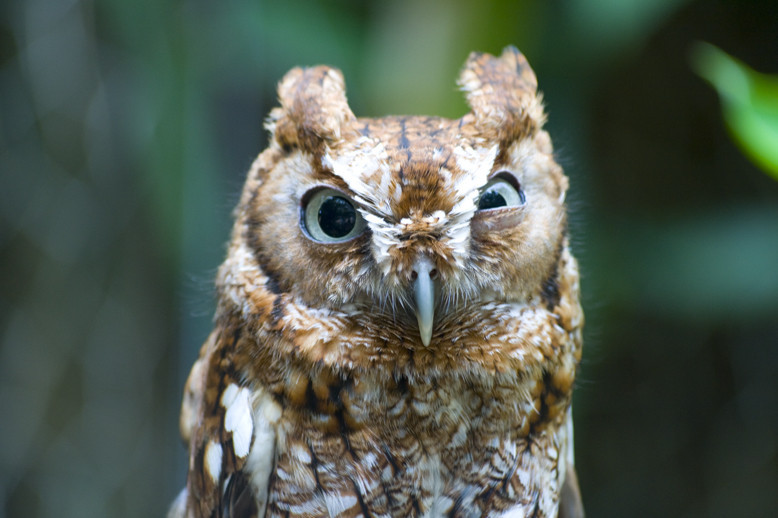
\includegraphics[width=0.49\textwidth]{./Figs/placeholder.jpeg}
        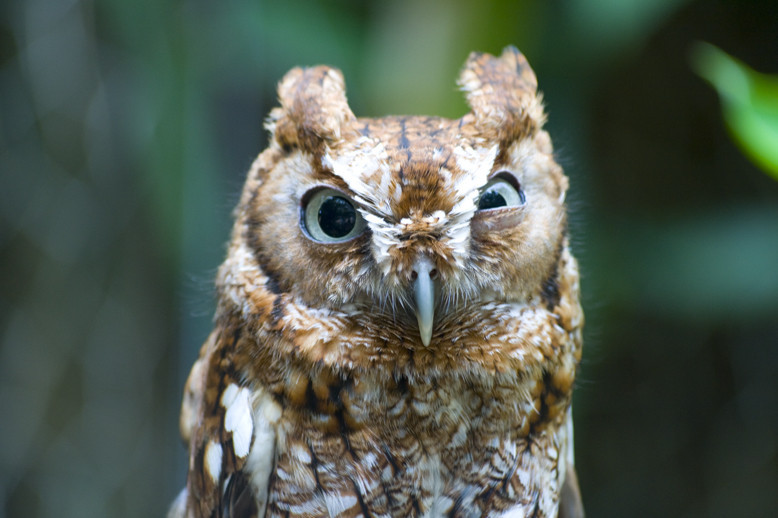
\includegraphics[width=0.49\textwidth]{./Figs/placeholder.jpeg}

    \caption{BDT response for training and testing samples of signal and background decays for the adaptive boost BDT (left) and the uBoost BDT (right). }
    \label{fig:ELBDTovertrain}
\end{figure}



%\begin{figure}[htbp]
%   \centering
%        \includegraphics[width=0.6\textwidth]{./Figs/Appendix2/}
%    \caption{BDT response for training and testing samples of signal and background decays for the global BDT~cite{}. }
%    \label{fig:BFBDTovertrain}
%\end{figure}



